\iffalse
    \title{Assignment}
    \author{EE24BTECH11063}
    \section{ce}
    \chapter{2012}
  \fi

\item \textbf{Question Number: 1 Question Type : MCQ}\\
Choose the appropriate word/phrase, out of the four options given below, to complete the sentence:\\
\\
Apparent lifelessness \rule{1cm}{0.15mm} dormant life.
\begin{enumerate}
    \begin{multicols}{4}
        \item harbours
        \item leads to
        \item supports
        \item affects
    \end{multicols}
\end{enumerate}
\bigskip
\item \textbf{Question Number: 2 Question Type : MCQ}\\
Fill in the blank with the correct idiom/phrase\\
\\
That boy from the town was a \rule{1cm}{0.15mm} in the sleepy village.
\begin{enumerate}
    \begin{multicols}{2}
        \item dog out of forward
        \columnbreak
        \item sheep from the heap
    \end{multicols}
    \begin{multicols}{2}
        \item fish out of water
        \item bird from the flock
    \end{multicols}
\end{enumerate}
\bigskip
\item \textbf{Question Number: 3 Question Type : MCQ}\\
 Choose the statement where underlined word is used correctly. \\

\begin{enumerate}
    \item When the teacher eludes to different authors, he is being \underline{elusive}.
    \item When the thief keeps eluding the police, he is being \underline{elusive}.
    \item Matters that are difficult to understand, identify or remember are \underline{allusive}.
    \item Mirages can be \underline{allusive}, but a better way to express them is illusory.
\end{enumerate}
\bigskip
\item \textbf{Question Number: 4 Question Type : MCQ}\\
Tanya is older than Eric. \\
Cliff is older than Tanya. \\
Eric is older than Cliff. \\

 \setlength\parindent{24pt} If the first two statements are true, then the third statement is: \\

\begin{enumerate}
    \item True
    \item False
    \item Uncertain
    \item Data insufficient
\end{enumerate}
\bigskip
\item \textbf{Question Number: 5 Question Type : MCQ}\\
Five teams have to compete in a league, with every team playing every other team exactly once, before going to the next round. How many matches will have to be held to complete the league round of matches? \\

\begin{enumerate}
\begin{multicols}{4}
    \item 20
    \item 10
    \item 8
    \item 5
\end{multicols}
\end{enumerate}
\bigskip
\section*{Q.6 to Q.10 carry 2 marks each}
\item \textbf{Question Number: 6 Question Type : MCQ}\\
Select the appropriate option in place of the underlined part of the sentence. \\
\\
\underline{Increased productivity necessary} reflects greater efforts made by the employees. \\

\begin{enumerate}
    \item Increase in productivity necessary
    \item Increase productivity is necessary
    \item Increase in productivity necessarily
    \item No improvement required
\end{enumerate}
\bigskip
\item \textbf{Question Number: 7 Question Type : MCQ}\\
Given below are two statements followed by two conclusions. Assuming these statements to be true, decide which one logically follows. \\

\textbf{Statements:}
\begin{enumerate}
    \item[I.] No manager is a leader.
    \item[II.] All leaders are executives.
\end{enumerate}

\textbf{Conclusions:}
\begin{enumerate}
    \item[I.] No manager is an executive.
    \item[II.] No executive is a manager.
\end{enumerate}

\begin{enumerate}
    \item Only conclusion I follows.
    \item Only conclusion II follows.
    \item Neither conclusion I nor II follows.
    \item Both conclusions I and II follow.
\end{enumerate}
\bigskip
\item \textbf{Question Number: 8 Question Type : NAT}\\
In the given figure$\ref{fig:1}$ angle $ Q $ is a right angle, $ PS:QS = 3:1 $, $ RT:QT = 5:2 $ and $ PU:UR = 1:1 $. If the area of triangle $ QTS $ is $ 20 \, \text{cm}^2 $, then the area of triangle $ PQR $ in $ \text{cm}^2 $ is \rule{1cm}{0.15mm}.
\begin{figure}[H]
    \centering
    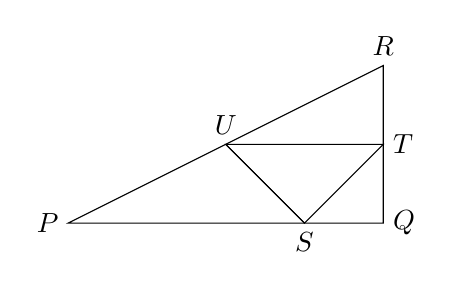
\begin{tikzpicture}
\draw (0,0) node[left] {$P$} -- (4,0) node[right] {$Q$} -- (4,2) node[above] {$R$} -- cycle;
\draw (3,0) node[below] {$S$} -- (2,1) node[above] {$U$} -- (4,1) node[right] {$T$} -- cycle;
\draw (2,1) -- (3,0);
\end{tikzpicture}
    \caption{}
    \label{fig:1}
\end{figure}
\bigskip
\item \textbf{Question Number: 9 Question Type : MCQ}\\
Right triangle $ PQR $ is to be constructed in the $ xy $-plane so that the right angle is at $ P $ and line $ PR $ is parallel to the x-axis. The x and y coordinates of $ P, Q, $ and $ R $ are to be integers that satisfy the inequalities: $ -4 \leq x \leq 5 $ and $ 6 \leq y \leq 16 $. How many different triangles could be constructed with these properties? \\

\begin{enumerate}
\begin{multicols}{4}
    \item 110
    \item 1,100
    \item 9,900
    \item 10,000
    \end{multicols}
\end{enumerate}
\bigskip
\item \textbf{Question Number: 10 Question Type : MCQ}\\
A coin is tossed thrice. Let $ X $ be the event that heads occur in each of the first two tosses. Let $ Y $ be the event that a tail occurs on the third toss. Let $ Z $ be the event that two tails occur in three tosses. Based on the above information, which one of the following statements is TRUE? \\

\begin{enumerate}
    \item $ X $ and $ Y $ are not independent
    \item $ Y $ and $ Z $ are dependent
    \item $ Y $ and $ Z $ are independent
    \item $ X $ and $ Z $ are independent
\end{enumerate}
\bigskip
\section*{Q.11 to Q.35 carry 1 mark each}
\item \textbf{Question Number: 11 Question Type : NAT}\\
Let $ T : \mathbb{R}^4 \to \mathbb{R}^4 $ be a linear map defined by \\

$T(x, y, z, w) = (x + z, 2x + y + 3z, 2y + 2z).$

Then the rank of $ T $ is equal to \rule{1cm}{0.15mm}
\bigskip
\item \textbf{Question Number: 12 Question Type : NAT}\\
Let $ M $ be a $ 3 \times 3 $ matrix and suppose that $ 1, 2 $, and $ 3 $ are the eigenvalues of $ M $. If 

$M^{-1} = \frac{M^2}{\alpha} - M + \frac{11}{\alpha} I_3$

for some scalar $ \alpha \neq 0 $, then $ \alpha $ is equal to \rule{1cm}{0.15mm}.
\bigskip
\item \textbf{Question Number: 13 Question Type : NAT}\\
Let $ M $ be a $ 3 \times 3 $ singular matrix and suppose that $ 2 $ and $ 3 $ are eigenvalues of $ M $. Then the number of linearly independent eigenvectors of 

$M^3 + 2M + I_3$

is equal to \rule{1cm}{0.15mm}.

